\documentclass[10pt,a4paper]{article}
\usepackage[a4paper, total={6in, 9in}]{geometry}
\usepackage[latin1]{inputenc}
\usepackage{amsmath}
\usepackage{amsfonts}
\usepackage{amssymb}
\usepackage{mathtools}
\usepackage{graphicx}
\usepackage{float}
\usepackage[usenames, dvipsnames]{color}
\usepackage{fancyhdr}
\usepackage{enumitem}
\usepackage{listings}
\setlength{\headheight}{15.2pt}
\pagestyle{fancy}
\setlength{\parindent}{0em}
\setlength{\parskip}{10pt}
\setlist[enumerate,1]{label=\alph*)}
\setlist[enumerate,2]{label=(\roman*)}
\definecolor{LGray}{gray}{0.9}
\definecolor{DGray}{gray}{0.4}
\usepackage{inconsolata}
\usepackage[T1]{fontenc}
\lstset{language=python, tabsize=2, breaklines=true, postbreak=\mbox{\textcolor{red}{$\hookrightarrow$}\space}, basicstyle=\linespread{0.7}\ttfamily, commentstyle=\color{DGray}} 
\newcommand*\diff{\mathop{}\!\mathrm{d}}
\lstset{showstringspaces=false}



\begin{document}
\title{ENGSCI762 A3}
\author{Benjamin Yi}
\rhead{Benjamin Yi - byi649 - 925302651}
\lhead{ENGSCI762 A3}

\section*{Question 1}
\begin{enumerate}
\item
\begin{lstlisting}[language=VBscript]
Sub main()
	Dim col As Integer, num As Integer, cell As Integer, adj(0 To 3) As Integer
	Application.Calculation = xlManual
	For cell = 0 To 27 'Iterate across blocks
		num = 0
		If Int(cell / 7) <> 0 Then adj(num) = cell - 7: num = num + 1 'If not on top edge, add above cell to adjacents
		If Int(cell / 7) <> 3 Then adj(num) = cell + 7: num = num + 1 'If not on bottom edge, add below cell to adjacents
		If cell Mod 7 <> 0 Then adj(num) = cell - 1: num = num + 1 'If not on left edge, add left cell to adjacents
		If cell Mod 7 <> 6 Then adj(num) = cell + 1: num = num + 1 'If not on right edge, add right cell to adjacents
		generateColumns cell, col, adj, num
	Next cell
	Application.Calculation = xlAutomatic
End Sub

Sub generateColumns(cell As Integer, col As Integer, adj() As Integer, num As Integer)
	Dim m As Integer
	For m = 0 To 2 ^ num - 1 'For each centre permutation
		Sheet1.Cells(cell + 1, col + 1) = 1 'Deliver to self
		For n = 0 To num - 1
			If (m And (2 ^ n)) <> 0 Then Sheet1.Cells(adj(n) + 1, col + 1) = 1 'Deliver to adjacents
		Next n
		col = col + 1
	Next m
End Sub
\end{lstlisting}

\item 
The A matrix consists of 28 rows, one for each block, and 288 columns. Each column corresponds to a binary variable that is equal to one if the set described by the column is chosen and zero otherwise.

\begin{figure}[H]
	\centering
	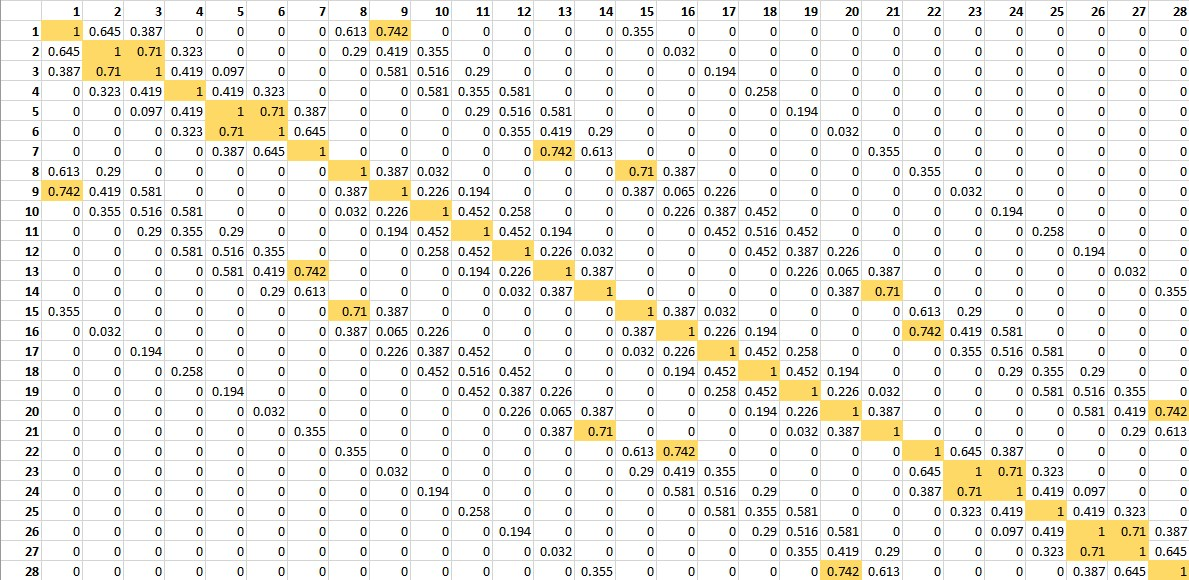
\includegraphics[width=1\linewidth]{texstudio_Thursday-31-May-21'04'00}
	\caption{Sum of fractions table - highlighted yellow are numbers close to 1}
	\label{fig:texstudiothursday-31-may-210400}
\end{figure}

\item 
\begin{enumerate}
	\item 1-branch:
	\begin{align*}
		x_i \leq 0 \quad \forall i \in \text{I}^*(s, t) \text{ where } \text{I}^*(s, t) = \{i | (a_{si} = 1, a_{ti} = 0) \text{ or } (a_{si} = 0, a_{ti} = 1)\}
	\end{align*}
	\item 0-branch:
	\begin{align*}
	x_i \leq 0 \quad \forall i \in \text{I}(s, t) \text{ where } \text{I}(s, t) = \{i | (a_{si} = 1, a_{ti} = 1)\}
	\end{align*}
\end{enumerate}

\item 
Branching on the pair (0, 8): \\
0-branch: z = 44107 \\
1-branch: z = 43340 (integer)

\item 
Yes, the optimal solution is the solution from the 1-branch, as it is integer. The solution is as follows, with a total cost of \$43340:

\begin{tabular}{|c|c|c|c|}
	\hline 
	Cabinet & Location & Battery size (mAh) & Delivers to \\ 
	\hline 
	1 & 1 & 5000 & 1, 2, 3, 9 \\ 
	\hline 
	2 & 4 & 3000 & 4, 5, 11 \\ 
	\hline 
	3 & 7 & 5000 & 0, 7, 8, 14 \\ 
	\hline 
	4 & 13 & 5000 & 6, 12, 13, 20 \\ 
	\hline 
	5 & 17 & 5000 & 10, 16, 17, 18, 24 \\ 
	\hline 
	6 & 22 & 5000 & 15, 21, 22, 23 \\ 
	\hline 
	7 & 26 & 5000 & 19, 25, 26, 27 \\ 
	\hline 
\end{tabular} 
\end{enumerate}

\section*{Question 2}
\begin{enumerate}
\item
Order the deliveries by shortest distance first, then deliver in that order.

\item 
The GSPP is formulated as such:
\begin{align*}
\text{min}& \qquad z = c^Tx \\
\text{st}& \qquad Ax = 1 \\
& \qquad e^Tx \leq 14 \\
& \qquad x \text{  binary}
\end{align*}
where A and x are defined as per the standard SPP, and \(e^T\) is the vector of ones.\\
The extra constraint line restricts the total number of cabinets installed to be less than 14, and the RHS is adjusted to produce a range of non-dominated solutions.

The code used to generate the A matrix:
\lstinputlisting{generateA.py}
This generates all potential combinations of neighbours around a cabinet that are formed from the 8 nearest blocks, between lengths 3 and 5 inclusive. \\ \\
This will give an A matrix of column length 5004. By choosing neighbours only from the 8 closest blocks and restricting the length of the set to be between 3 and 5, this is much lower than enumerating all possible combinations - which would be \(2^{48}\) in total. \\ \\
While technically choosing only the 8 closest neighbours and only choosing sets of length 3 or greater potentially cuts off the optimal solution, the remaining solutions will tend to have much better objective functions than the rest of the sets. The chance of cutting off the optimal solution is low, and the computational costs recuperated are high (Excel cannot support \(2^{48}\) columns in a worksheet), so it is worth doing.

\item 
As this is a bi-objective optimisation problem, it has been solved for all feasible monetary costs, optimising average delivery time each time.\\ \\
Number of cabinets: 14, cost = \$84000, average time taken: 256 seconds\\ \\
\begin{tabular}{|c|c|}
	\hline 
	Cabinet location & Delivers to \\ 
	\hline 
	551500 & 551100, 551200, 551500, 551600 \\ 
	\hline 
	551401 & 551300, 551401, 551402, 551700 \\ 
	\hline 
	552600 & 552500, 552600, 552700, 553600 \\ 
	\hline 
	552900 & 552400, 552800, 552900, 553200 \\ 
	\hline 
	553100 & 553000, 553100, 553400 \\ 
	\hline 
	555200 & 553300, 555100, 555200 \\ 
	\hline 
	559100 & 556100, 559100, 559200 \\ 
	\hline 
	556400 & 556200, 556300, 556400, 556800 \\ 
	\hline 
	556900 & 556500, 556900, 557800 \\ 
	\hline 
	557000 & 556600, 557000, 557200 \\ 
	\hline 
	557300 & 557100, 557300, 557401, 557402 \\ 
	\hline 
	557600 & 557500, 557600, 558600 \\ 
	\hline 
	557900 & 557700, 557900, 558100 \\ 
	\hline 
	558200 & 558000, 558200, 558500 \\ 
	\hline 
\end{tabular} \\ \\
Visualisation:
\begin{figure}[H]
	\centering
	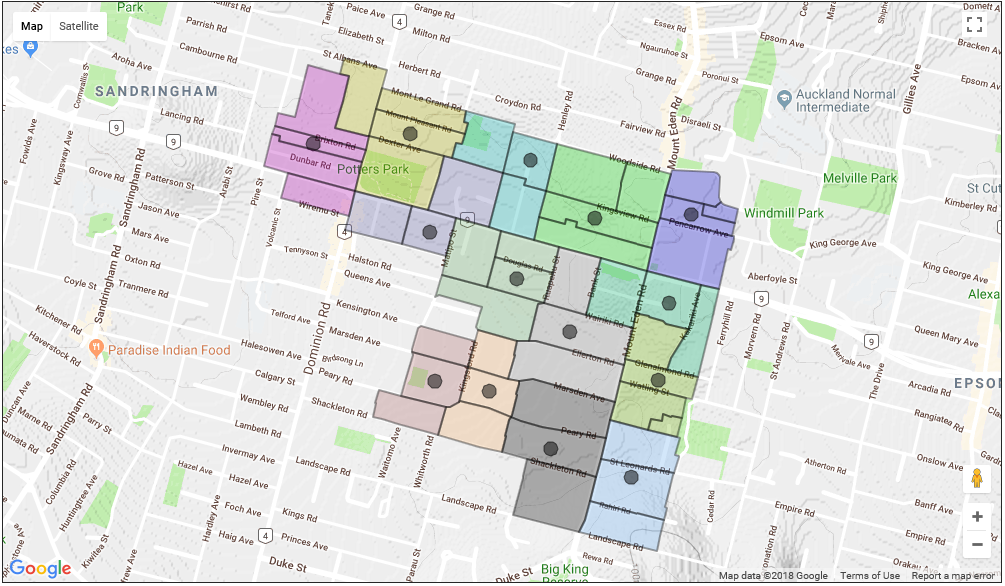
\includegraphics[width=0.7\linewidth]{14}
	\caption{Cabinet distribution for 14 cabinets}
	\label{fig:14}
\end{figure}


Number of cabinets: 13, cost = \$78000, average time taken: 279 seconds\\ \\
\begin{tabular}{|c|c|}
	\hline 
	Cabinet location & Delivers to \\ 
	\hline 
	551500 & 551100, 551200, 551500, 551600 \\ 
	\hline 
	551401 & 551300, 551401, 551402, 551700 \\ 
	\hline 
	552600 & 552500, 552600, 552700, 553600 \\ 
	\hline 
	552900 & 552400, 552800, 552900, 553200 \\ 
	\hline 
	553100 & 553000, 553100, 553400 \\ 
	\hline 
	555200 & 553300, 555100, 555200 \\ 
	\hline 
	559100 & 556100, 559100, 559200 \\ 
	\hline 
	556400 & 556200, 556300, 556400, 556800 \\ 
	\hline 
	556900 & 556500, 556600, 556900, 557800 \\ 
	\hline 
	557100 & 557000, 557100, 557200, 557300 \\ 
	\hline 
	557500 & 557401, 557402, 557500, 557600 \\ 
	\hline 
	557900 & 557700, 557900, 558000, 558100 \\ 
	\hline 
	558500 & 558200, 558500, 558600 \\ 
	\hline 
\end{tabular} \\ \\

Number of cabinets: 12, cost = \$72000, average time taken: 305 seconds\\ \\
\begin{tabular}{|c|c|}
	\hline 
	Cabinet location & Delivers to \\ 
	\hline 
	551500 & 551100, 551200, 551500, 551600 \\ 
	\hline 
	551401 & 551300, 551401, 551402, 551700 \\ 
	\hline 
	552600 & 552500, 552600, 552700, 553600 \\ 
	\hline 
	552900 & 552400, 552800, 552900, 553200 \\ 
	\hline 
	553400 & 553000, 553100, 553400, 556300 \\ 
	\hline 
	555200 & 553300, 555100, 555200, 556200 \\ 
	\hline 
	559100 & 556100, 558100, 559100, 559200 \\ 
	\hline 
	556900 & 556500, 556600, 556900, 557800 \\ 
	\hline 
	557100 & 557000, 557100, 557200, 557300 \\ 
	\hline 
	557500 & 557401, 557402, 557500, 557600 \\ 
	\hline 
	558200 & 558000, 558200, 558500, 558600 \\ 
	\hline 
	557700 & 556400, 558600, 557700, 557900 \\ 
	\hline 
\end{tabular} \\ \\

Number of cabinets: 11, cost = \$66000, average time taken: 340 seconds\\ \\
\begin{tabular}{|c|c|}
	\hline 
	Cabinet location & Delivers to \\ 
	\hline 
	551500 & 551100, 551500, 551600, 553100 \\ 
	\hline 
	551401 & 551200, 551300, 551401, 551402, 551700 \\ 
	\hline 
	552600 & 552400, 552500, 552600, 552700, 553600 \\ 
	\hline 
	552900 & 552800, 552900, 553000, 553200 \\ 
	\hline 
	555200 & 553300, 555100, 555200, 556200 \\ 
	\hline 
	559100 & 556100, 557900, 558100, 559100, 559200 \\ 
	\hline 
	556400 & 553400, 556300, 556400, 556500, 556800 \\ 
	\hline 
	556900 & 556600, 556900, 557700, 557800 \\ 
	\hline 
	557100 & 557000, 557100, 557200, 557300 \\ 
	\hline 
	557500 & 557401, 557402, 557500, 557600 \\ 
	\hline 
	558200 & 558000, 558200, 558500, 558600 \\ 
	\hline 
\end{tabular} \\ \\

Number of cabinets: 10, cost = \$60000, average time taken: 378 seconds\\ \\
\begin{tabular}{|c|c|}
	\hline 
	Cabinet location & Delivers to \\ 
	\hline 
	551401 & 551200, 551300, 551401, 551402, 551700 \\ 
	\hline 
	551600 & 551100, 551500, 551600, 556500, 556600 \\ 
	\hline 
	552900 & 552400, 552800, 552900, 553200 \\ 
	\hline 
	552700 & 552500, 552600, 552700, 553600, 555100 \\ 
	\hline 
	553300 & 553000, 553100, 553300, 553400, 555200 \\ 
	\hline 
	559100 & 556100, 557900, 558100, 559100, 559200 \\ 
	\hline 
	556400 & 556200, 556300, 556400, 556800, 557700 \\ 
	\hline 
	557100 & 556900, 557000, 557100, 557200, 557300 \\ 
	\hline 
	557500 & 557401, 557402, 557500, 557600, 558600 \\ 
	\hline 
	558000 & 557800, 558000, 558200, 558500 \\ 
	\hline 
\end{tabular} \\ \\

Each solution trades off monetary cost and average time for delivery, therefore none of these solutions are strictly superior to any other. The choice will depend on whatever objective the decision maker deems more important.
\end{enumerate}
\end{document}

